\pdfminorversion=4
\documentclass[aspectratio=169]{beamer}
\usepackage{verbatim}
\newenvironment{metaverbatim}{\verbatim}{\endverbatim}
\usepackage{courier}
\usepackage{lmodern}
\usepackage{apacite}
\usepackage{xcolor}
\xdefinecolor{azulcesafuerte}{HTML}{14387e}
\xdefinecolor{azulcesaclaro}{HTML}{7ab6e0}
\xdefinecolor{azulcesamedio}{HTML}{0A72BC}

\usetheme{Madrid}
%\usecolortheme[named=black]{structure}
%
\setbeamercolor{normal text}{fg=azulcesafuerte}
\setbeamercolor{background canvas}{bg=white}
\setbeamercolor{frametitle}{fg=white, bg=azulcesafuerte}
\setbeamercolor{section in toc}{fg=azulcesaclaro}
\setbeamercolor{navigation symbols}{}

\setbeamertemplate{background}{\tikz[overlay,remember picture]\node[opacity=0.15]at (current page.center){\includegraphics[width=14.7cm]{}};}
\usepackage{tikz}
\usepackage{kantlipsum}
\setbeamercolor*{title}{fg=white, bg=azulcesafuerte}
\setbeamercolor{titlelike}{parent=structure}

\setbeamercolor*{palette primary}{bg=azulcesafuerte,fg=white}
\setbeamercolor*{palette secondary}{bg=azulcesafuerte,fg=white}
\setbeamercolor*{palette tertiary}{bg=azulcesafuerte,fg=white}

% Change base colour beamer@blendedblue (originally RGB: 0.2,0.2,0.7)
\colorlet{beamer@blendedblue}{azulcesaclaro}
\usepackage[english]{babel}
\usepackage{apacite}
\usepackage{marvosym}
\usepackage{subfig}
\usepackage{graphicx}
\usepackage[utf8x]{inputenc}
\usepackage{url}
\usepackage{hyperref}
\usepackage{times}
\usepackage{pxfonts}
\usepackage{fontenc}
%\usepackage[dvipsnames]{xcolor}
\setbeamertemplate{bibliography item}[text]
\title[Analítica de Datos para los Negocios]{Analítica de Datos para Los Negocios}

\author[Prof. Juan C. Correa, Ph.D.]{Prof. Juan C. Correa, Ph.D.}

\institute[]{
Colegio de Estudios Superiores de Administración\\
Bogotá - Colombia\\
% \color{azulcesaclaro}\Email  \href{mailto:juan.correan@cesa.edu.co}{juan.correan@cesa.edu.co}
}
\pgfdeclareimage[height=0.6cm]{OL}{OL}
 \logo{\pgfuseimage{OL}}
 \setbeamertemplate{caption}[numbered]
\date[Bogotá, Julio, 2021] % (optional)
{}

\subject{}
\begin{document}
\begin{frame}
\titlepage
\end{frame}

% \begin{frame}
% \frametitle{Agenda} 
% \tableofcontents
% \end{frame}

\begin{frame}
\begin{figure}
\centering
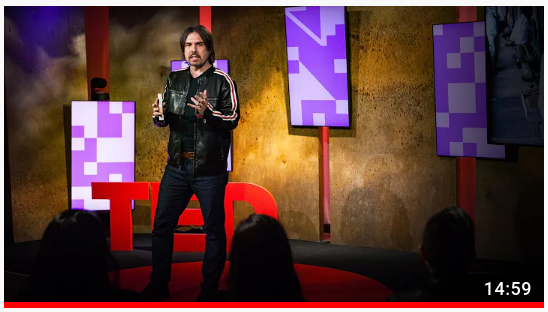
\includegraphics[width=.8\textwidth]{Cesar.png}
\end{figure}
\centering
\textcolor{blue}{\url{https://youtu.be/UUp39T3fPAo}}
\end{frame}


\begin{frame}{Presentación del Curso}
Los \textbf{datos de  valor para los negocios} están por doquier \cite{Shmueli2020}.\\
\vspace{0.3cm}
\begin{itemize}
\pause
\item \href{https://www.seatguru.com/}{\textcolor{blue}{seatguru.com}} muestra datos realistas sobre la experiencia del pasajero para su próximo vuelo con una aerolínea específica.
\pause
\item \href{https://www.booking.com/}{\textcolor{blue}{booking.com}} muestra ofertas de alojamiento con comentarios de clientes que describen su experiencia como usuarios de estas instalaciones.
\pause
\item En \href{https://www.amazon.com/}{\textcolor{blue}{Amazon}}, \href{https://www.mercadolibre.com/}{\textcolor{blue}{mercadolibre}}, o \href{https://www.rappi.com/}{\textcolor{blue}{rappi}} los clientes evalúan el servicio recibido y publican sus opiniones  sobre productos y servicios. 
\end{itemize}
\pause
\vspace{0.3cm}
El futuro administrador de empresas debe comprender el valor y la utilidad de estos datos para proponer cambios estratégicos en la gestión productiva de los negocios o dirigir procesos de mejora contínua sustentando sus decisiones en datos relevantes.
\end{frame}

\begin{frame}{Presentación del Curso}
El curso de analítica de datos responde a estos desafíos mediante la aplicación de técnicas y herramientas modernas en la preparación, manipulación, exploración, análisis y visualización de datos, brindando al participante una visión amplia y completa sobre la gestión de la información para liderar y tomar decisiones basada en ella.
\end{frame}

\section{Los Negocios y Las Nuevas Tecnologías}
\begin{frame}
\begin{center}
\Huge
\textcolor{azulcesaclaro}{1\\
--------------------------------\\
Los Negocios y Las Nuevas Tecnologías}
\end{center}
\end{frame}


\begin{frame}
\begin{figure}
\centering
 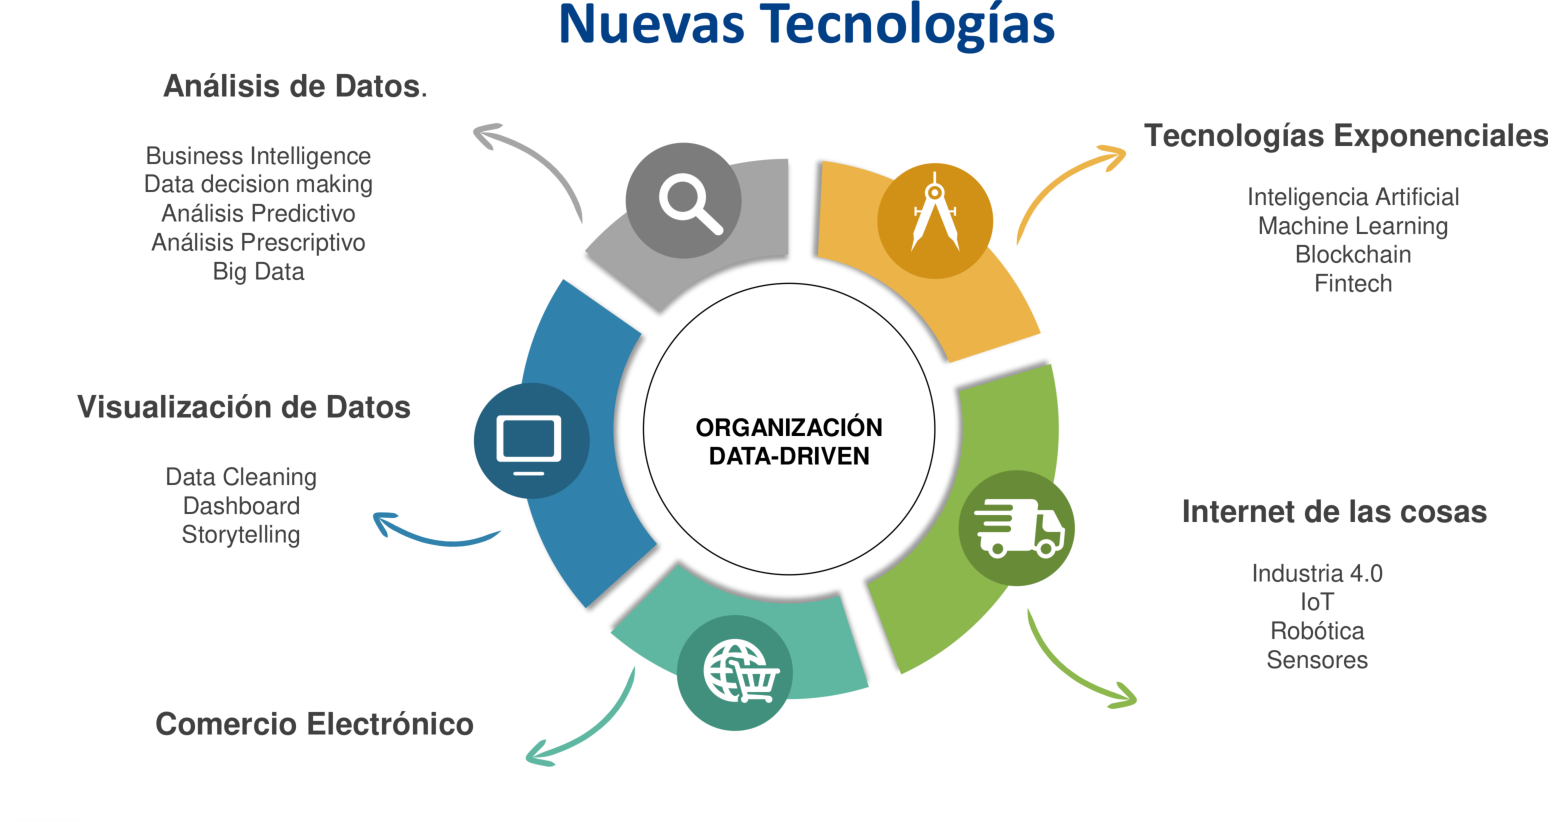
\includegraphics[width=.8\textwidth]{F1.pdf}
\end{figure}
\end{frame}

\begin{frame}
\begin{figure}
\centering
 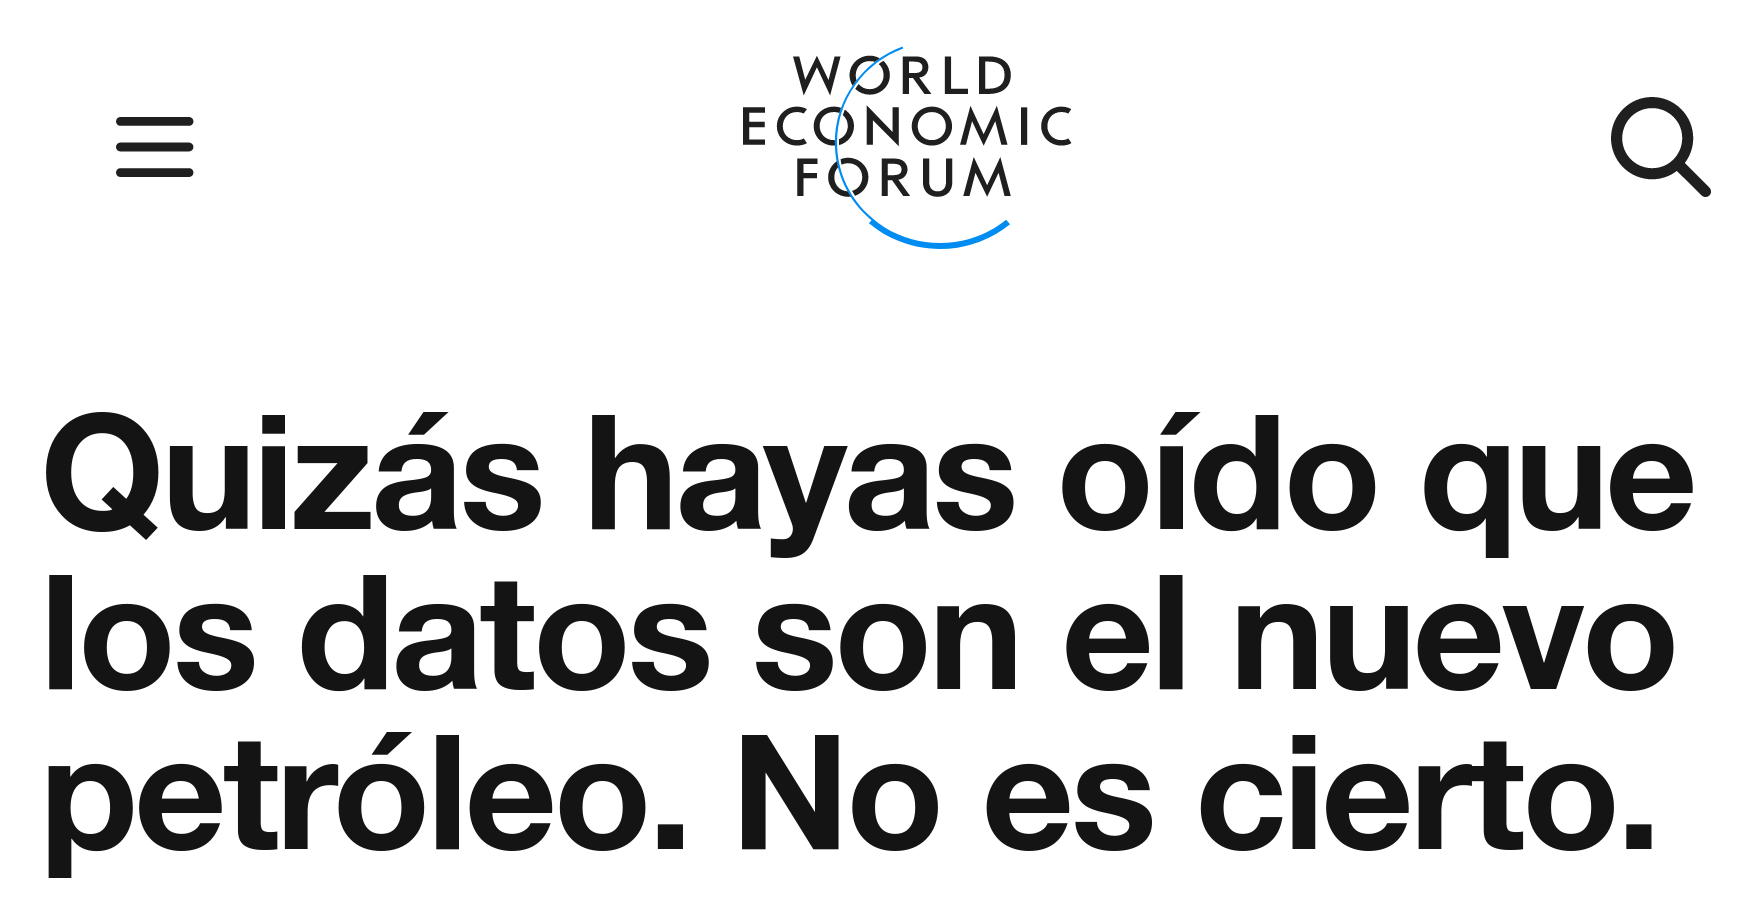
\includegraphics[width=.8\textwidth]{wef.png}
\end{figure}
\tiny{
\textcolor{blue}{\url{https://es.weforum.org/agenda/2018/01/quizas-hayas-oido-que-los-datos-son-el-nuevo-petroleo-no-es-cierto/}}}
\end{frame}

\subsection{El Valor de Los Datos}

\begin{frame}
\begin{center}
\Huge
\textcolor{azulcesaclaro}{1.1\\
--------------------------------\\
El valor de los datos}
\end{center}
\end{frame}

\begin{frame}
Aunque a cada segundo cualquier persona con conexión a Internet a través de su teléfono celular u otro dispositivo está generando data potencialmente valiosa, ésta no tiene valor per se.\\
\vspace{0.5cm}
El valor de los datos se obtiene de un cuidadoso y elaborado proceso de extracción de información y descubrimiento de conocimiento. Este proceso se apoya en el concepto de \textbf{Jerarquía de la Sabiduría} \cite{Rowley2007}
\end{frame}

\begin{frame}
\begin{figure}
\centering
 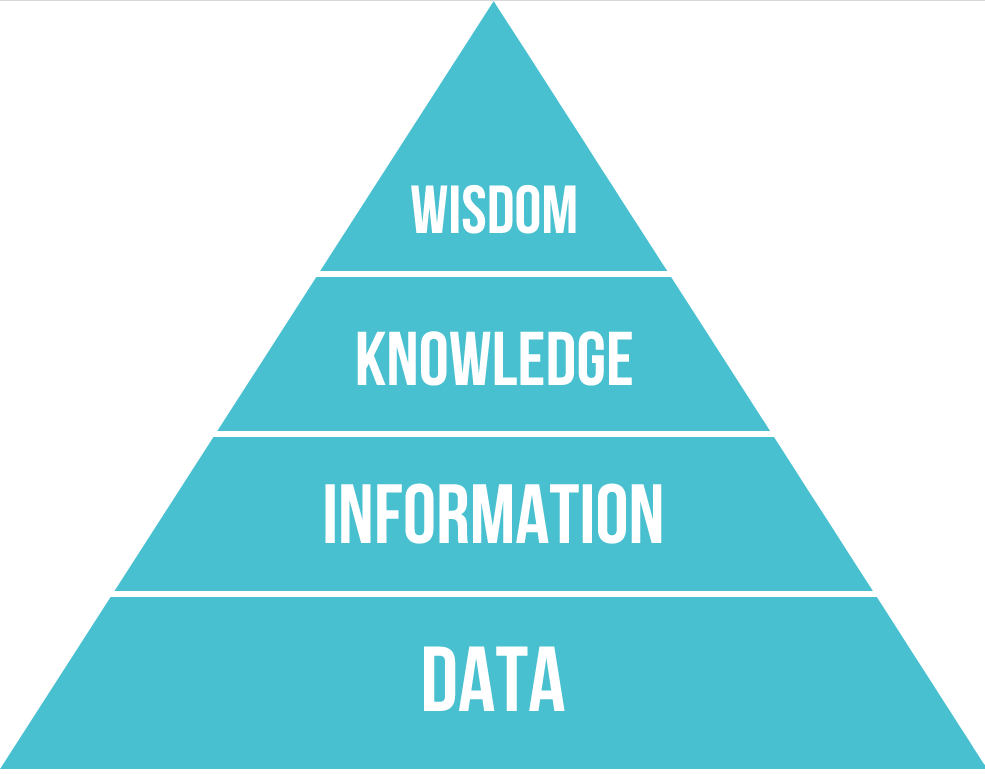
\includegraphics[width=.5\textwidth]{dikw.png}
\end{figure}
Con la \textbf{Jerarquía de la Sabiduría} no se debe confundir el concepto de datos, del concepto de información, del conocimiento y la sabiduría \cite{Zins2007}.
\end{frame}

\subsection{El rol de los futuros gerentes}
\begin{frame}
\begin{center}
\Huge
\textcolor{azulcesaclaro}{1.2\\
--------------------------------\\
El Rol de los Futuros Gerentes}
\end{center}
\end{frame}

\begin{frame}
En la era de la llamada \textbf{Industria 4.0}, los futuros gerentes deben ser especialmente sensibles a las nuevas tendencias del consumidor. También deben conocer lo que están haciendo sus competidores por captar nuevos clientes y retener a clientes habituales (e.g., análisis de voz-a-voz, marketing experiencial, promociones personalizadas, minería de datos por Internet, Internet de las cosas).  \\
\vspace{0.5cm}
Tareas como las anteriores solo pueden ejecutarse con apoyo de estrategias orientadas a la extracción de información y descubrimiento de conocimiento, lo cual requiere desarrollar varias habilidades y experticias.
\end{frame}

\begin{frame}
\centering
\begin{figure}
\centering
 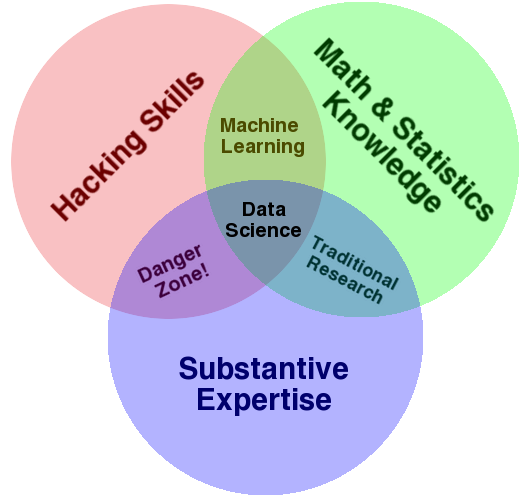
\includegraphics[width=.45\textwidth]{hacking.png}
\end{figure}
Tomado de Edvancer Eduventures\\ \textcolor{blue}{\url{https://www.edvancer.in/8-data-science-skills/}}
\end{frame}

\section{Aplicaciones Reales}
\begin{frame}
\begin{center}
\Huge
\textcolor{azulcesaclaro}{2\\
--------------------------------\\
Aplicaciones Reales}
\end{center}
\end{frame}

\begin{frame}
\begin{itemize}
\item \textbf{Industria Automotriz}: Predicción de daños en accidentes vehiculares \cite{Belaid2021}
\vspace{0.6cm}
\pause
\item \textbf{Industria de Servicios en Consumo Masivo}: Análisis del cumplimiento en entrega de domicilios de comida \cite{Correa2019}
\pause
\vspace{0.6cm}
\item \textbf{Industria de Comunicaciones y Divulgación Científica}: El impacto de la piratería para el acceso al conocimiento técnico-científico \cite{Correa2021}
\end{itemize}
\end{frame}


\begin{frame}
 \begin{figure}
\centering
 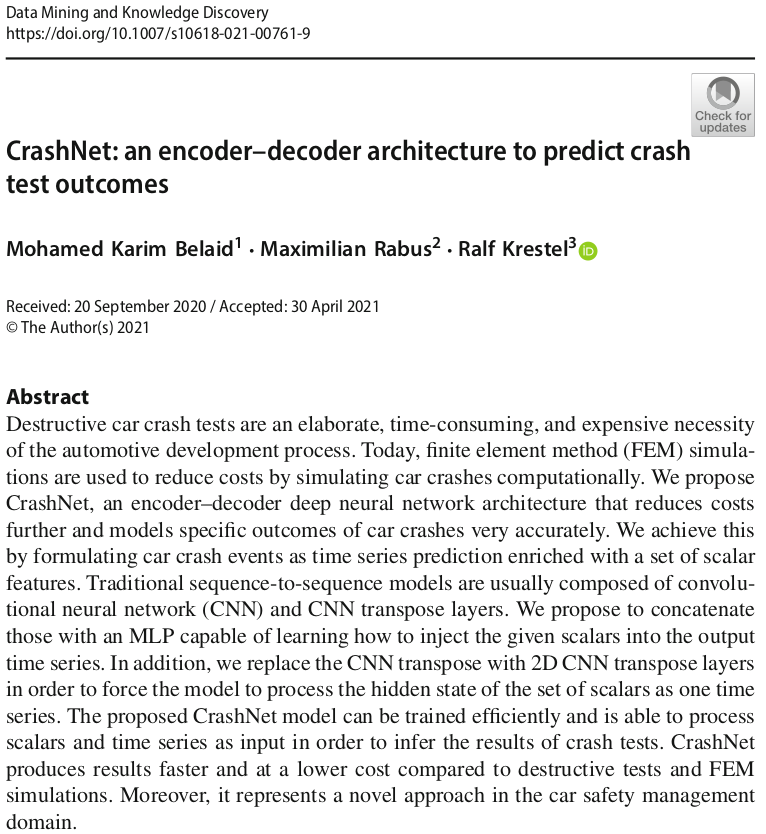
\includegraphics[width=.5\textwidth]{Ejemplo1.png}
\end{figure}  
\end{frame}

\begin{frame}
 \begin{figure}
\centering
 \includegraphics[width=.7\textwidth]{Ejemplo2.png}
\end{figure}  
\cite{Correa2019}
\end{frame}

\begin{frame}
 \begin{figure}
\centering
 
\includegraphics[width=.7\textwidth]{ejemplo3.png}
\end{figure}  
\cite{Correa2021}
\end{frame}

\section{Sugerencias para Aprender}
\begin{frame}
\begin{center}
\Huge
\textcolor{azulcesaclaro}{3\\
--------------------------------\\
Normativas del Curso y\\
Sugerencias para Aprender}
\end{center}
\end{frame}


\begin{frame}
\begin{itemize}
\item Las normativas y las políticas de este curso están explícitamente descritas en el syllabus de la asignatura y el estudiante se compromete a cumplirlas en cada sesión.
\vspace{0.5cm}
\item El curso contempla un total de 34 sesiones de clase. Se realizarán evaluaciones cortas y de dificultad moderada (iniciando con evaluaciones muy sencillas) en varias ocasiones a través de diferentes modalidades (i.e., talleres, ejercicios guiados, dos parciales y un examen final).
\end{itemize}    
\end{frame}

\begin{frame}
\begin{itemize}
\item Cada sesión de clases tiene un objetivo de aprendizaje. Tal objetivo será descrito explícitamente al inicio de cada clase. El estudiante siempre debe asegurarse de comprender la relación que existe entre la sesión de clases y el syllabus.
\vspace{0.5cm}
\item Se recomienda usar la presentación de cada clase como guía de estudio para las evaluaciones. Con estas presentaciones se sintetiza la información relevante de la bibliografía del curso y ofrecen pautas clave para un rendimiento  exitoso en cada evaluación.
\end{itemize}
\end{frame}

\begin{frame}
\begin{itemize}
\item Para sacarle el máximo provecho al curso se sugiere tener mucha concentración y orientación hacia los detalles que exigen las nuevas herramientas necesarias en la analítica de datos para los negocios (e.g., Python, RStudio, Jasp, SPSS).
\begin{figure}
\centering
 
\includegraphics[width=.5\textwidth]{tools2.png}
\end{figure}
\end{itemize}
\end{frame}

\begin{frame}
\begin{itemize}
\item Para asgurar el objetivo de aprendizaje de cada sesión, se sugiere observar los videos de las clases desarrolladas especialmente en aquellas donde se realizaron ejercicios guiados para el análisis de datos.
\end{itemize}
\end{frame}




% \begin{frame}
% \centering
% \textbf{Questions?}
% \begin{figure}
% \centering
%  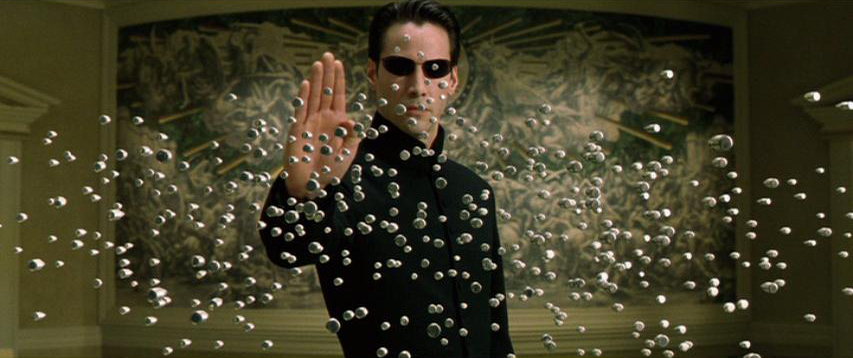
\includegraphics[width=1\textwidth]{Neo}
% \end{figure}
% \textbf{Shoot me!}
% \end{frame}


\section*{REFERENCIAS}
\begin{frame}[allowframebreaks]{Referencias}
\tiny{ 
\bibliographystyle{apacite}
\bibliography{REFS.bib}
} 
\end{frame}

\setbeamertemplate{background}{\tikz[overlay,remember picture]\node[opacity=1]at (current page.center){
\includegraphics[width=18cm]{ulam.png}};}
\pgfdeclareimage[height=0cm,width=0cm]{}{}
 \logo{\pgfuseimage{}}
\beamertemplatenavigationsymbolsempty
\begin{frame}
\end{frame}


\end{document}